\documentclass[a4paper,12pt]{article}
\usepackage{amssymb,amsmath,latexsym,enumerate}
\usepackage{mathtools}
\DeclarePairedDelimiter\ceil{\lceil}{\rceil}
\DeclarePairedDelimiter\floor{\lfloor}{\rfloor}
\usepackage{gensymb}
\usepackage{graphicx,graphics}%,floatflt}
\usepackage{exscale,cmmib57,mathrsfs}
\usepackage{color}
\usepackage{hyperref}
\usepackage{comment}
\usepackage[english]{babel}
\usepackage{natbib}
\usepackage{url}
\usepackage[utf8]{inputenc}
\usepackage{amsfonts,amsthm}
\usepackage{caption}
\usepackage{subcaption}
\usepackage{parskip}
\usepackage{fancyhdr}
\usepackage{vmargin}
\usepackage{xcolor}
\usepackage{lipsum}
\usepackage[T1]{fontenc}
\usepackage{geometry}
\setlength{\parskip}{1\parskip}

%%%%%%%%%%%%%%%%%%%%%%%%%%%%%%%%%%%%%%%%%%%%%%%%%%%%%%%%%%%%%%%%%
\fancypagestyle{plain}{
\fancyhf{}
\rfoot{\thepage}
\fancyfootoffset{0pt}
}
\makeatother
\pagestyle{fancy}
\fancyhf{}
\rfoot{\thepage}
\fancyfootoffset{0pt}
%%%%%%%%%%%%%%%%%%%%%%%%%%%%%%%%%%%%%%%%%%%%%%%%%%%%%%%%%%%%%%%

\geometry{a4paper,total={170mm,257mm},left=40mm,top=60mm,bottom=18mm}
%%%%%%%%%%%%%%%%%%%%%%%%%%%%%%%%%%%%%%%%%%%%%%%%%%%%%%%%

%%WATERMARK SETTINGS%%%%%%%%%%%%%%%%%%%%%%%%%%%%%%%%%%%%%%%%%%%%%%%%
\usepackage[printwatermark]{xwatermark}
\usepackage{draftwatermark}
\SetWatermarkAngle{0}
\SetWatermarkHorCenter{13cm}
\SetWatermarkVerCenter{17.3cm}
\SetWatermarkText{
\includegraphics[width=21cm,height=30cm]{WaterMark.png}}
%%%%%%%%%%%%%%%%%%%%%%%%%%%%%%%%%%%%%%%%%%%%%%%%%%%%%%%%%%%%%%%%%%%%%%%%%%
\author{e-Yantra Team} % Your name
\vspace{0.5cm}
\date{\normalsize\today} % Today's date or a custom date

%%%%%%%%%%%%%%%%%%%%%%%%%%%%%%%%%%%%%%%%%%%%%%%%%%%%%%%%%%%%%%%%%%%%%%%%%%%

\newtheorem{qstn}{Q}
\newcommand{\BQ}{\begin{qstn}\rm}
\newcommand{\EQ}{\end{qstn}}
\newtheorem{answ}{A}
\newcommand{\BA}{\begin{answ}\rm}
\newcommand{\EA}{\end{answ}}

%%%%%%%%%%%%%%%%%%%%%%%%%%%%%%%%%%%%%%%%%%%%%%%%%%%%%%%%%%%%%%%%%%
\begin{document}
\begin{center}
	\bf \Huge \underline{\textbf{Biped Patrol}} \\
	\vspace{5mm}
	\Large \underline {\textbf{Task 3.3: Think \& Answer}}\\
\end{center}
\vspace{5mm}
\begin{center}
	\begin{tabular}{|p{5cm}|p{10cm}|}
		\hline
		Team Id & \#1110 \\
		\hline
		College &  Guru Nanak Dev Engineering College, Ludhiana\\
		\hline
		Team Leader Name & Shubham Baranwal \\
		\hline
		e-mail & shubhambaranwal83@gmail.com \\
		\hline
		Date & \today \\
		\hline
	\end{tabular}
\end{center}
\vspace{25mm}
\begin{center}
	\begin{tabular}{|c|c|c|}
		\hline
		Question No. & Max. Marks & Marks Scored \\
		\hline
		Q1 &  10 & \\
		\hline
		Q2 &  20 & \\
		\hline
		Q3 &  5 & \\
		\hline
		Q4 &  5 & \\
		\hline
		Q5 &  5 & \\
		\hline
		Q6 &  10 & \\
		\hline
		Q7 &  15 & \\
		\hline
		Q8 &  8 & \\
		\hline
		Q9 &  4 & \\
		\hline
		Q10 &  8 & \\
		\hline
		Q11 &  10 & \\
		\hline
		Total &  100 & \\
		\hline
	\end{tabular}
\end{center}
\newpage 
\begin{center}
\bf \Huge \underline{\textbf{Biped Patrol}} \\
\vspace{5mm}
\Large \underline {\textbf{Task 3.3: Think \& Answer}}\\
\end{center}
\vspace{1cm}
\textbf{Instructions:}
\begin{itemize}
	\item There are no negative marks.
	\item Unnecessary explanation will lead to less marks even if answer is correct.
	\item If required, draw the image in a paper with proper explanation and add the snapshot in your corresponding answer.
\end{itemize}
\vspace{0.5cm}
\hrule height 0.5mm
\vspace{1cm}
%%%%%%%%%%%%%%%%%%%%%%%%%%%%%%%%%%%%%%%%%%%%%%%%%%%%%%%%%%%%%%%%%%
\BQ
Describe hardware design for the Medbot, your team is constructing. Describe various parts with well labeled image. Give reasons for selection of design.\hfill[10]
\EQ
\vspace{5mm}
\BA
%Write Your Answer Below This
Multi-layer design will be used by our team for the construction of our Medbot which will have 3 layer. First layer or the bottom layer will contain both the motors along with L298n motor driver. The second layer or the middle layer will contain xbee and ardunio mega along with buzzer and will be attached to frame which will hold the electromagnet which will be pointing downward direction so that it can pick the boxes. This design will be easy to control through LQR controller. We will place the battery on the top layer along with led to signal when required. The reason to place battery there is it will provide more weight at a height and this will increase the moment of inertia which will provide stability whenever there is torque.
So, our robot design should be selected.


\begin{figure}[h]
    \centering
    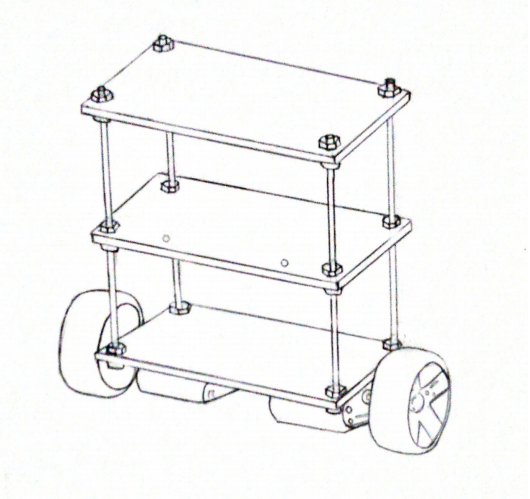
\includegraphics[width=0.35\textwidth]{robot.png}
    \caption{Robot Design}
    \label{fig:robot}
\end{figure}




\EA 
%%%%%%%%%%%%%%%%%%%%%%%%%%%%%%%%%%%%%%%%%%%%%%%%%%%%%%%%%%%%%%%%%%
%%%%%%%%%%%%%%%%%%%%%%%%%%%%%%%%%%%%%%%%%%%%%%%%%%%%%%%%%%%%%%%%%%
\vspace{5mm}
\BQ
In Task 1.2, you were asked to model different systems such as Simple Pulley, Complex Pulley, Inverted Pendulum with and without input and stabilizing the unstable equilibrium point using Pole Placement and LQR control techniques. There you had to choose the states; Derive the equations (usually non-linear), find equilibrium points and then linearize around the equilibrium points. You were asked to find out the linear system represented in the form 

\begin{equation} \label{Eqn1}
\dot{X}(t)=AX(t)+BU(t)
\end{equation}

Where $X(t)$ is a vector of all the state,i.e., $X(t)=[x_1(t),x_2(t),\dots,x_n(t)]^T$, and $U(t)$ is the vector of input to the system, i.e. $U(t)=[u_1(t),u_2(t),\dots,u_m(t)]^T$. $A$ is the State Matrix \& $B$ is the Input Matrix. \newline
In this question, you have to choose the states for the Medbot you are going to design. Model the system by finding out the equations governing the dynamics of the system using Euler-Lagrange Mechanics. Linearize the system via Jacobians around the equilibrium points representing your physical model in the form given in equation \ref*{Eqn1}. \\
\textbf{Note:} You may choose symbolic representation such as $M_w$ for Mass of wheel, etc. \hfill [20] 

\EQ
\vspace{5mm}
\BA
%Write Your Answer Below This
We can find the equation of motion governing the system using the Euler-Lagrange method 
$\frac{d}{dt}\left(\frac{\partial L}{\partial\dot{x}}\right)-\frac{\partial L}{\partial x}=0$, here $L=K.E.-P.E.$


So L is given by


    $L= \left[\frac{M_b}{2}+M_w+\frac{I_a}{R^2}\right]\dot{x}^2+\left[M_bd^2+\frac{1}{2}I_x\right]\dot{\phi}^2+\left[\left(M_w+\frac{I_a}{R^2}\right)L^2+\frac{1}{2}\left(I_zcos^2\phi+I_ysin^2\phi+M_bdsin^2\phi\right)\right]\dot{\psi}^2+M_bdcos\phi\dot{x}\dot{\phi}-\left[M_bgdcos\phi+M_bgR\right]$


So the final variables are \\
    $\ddot{x}=-\frac{M_b^2d^2gR^2}{\left(M_bd^2+I_x\right)\left(M_bR^2+2M_wR^2+2I_a\right)-\left(M_bdR\right)^2}\phi+\frac{R\left(M_bd^2+I_x+M_bdR\right)}{\left(M_bd^2+I_x\right)\left(M_bR^2+2M_wR^2+2I_a\right)-\left(M_bdR\right)^2}\left(\tau_1+\tau_2\right)$\\
    $\ddot{\phi}=\frac{\left(M_bR^2+2M_wR^2+2I_a\right)M_bgd}{\left[\left(M_b+2M_w\right)R^2+2I_a\right]I_x+2M_bd^2\left(M_wR^2+I_a\right)}\phi-\frac{\left(M_bR^2+2M_wR^2+2I_a\right)+M_bdR}{\left[\left(M_b+2M_w\right)R^2+2I_a\right]I_x+2M_bd^2\left(M_wR^2+I_a\right)}\left(\tau_1+\tau_2\right)$\\
    $\ddot{\psi}=\frac{L}{R\left[2\left(M_w+\frac{I_a}{R^2}\right)L^2+I_z\right]}\left(\tau_1-\tau_2\right)$\\
now considering $x(t)=\begin{bmatrix}x&\dot{x}&\phi&\dot{\phi}&\psi&\dot{\psi}\end{bmatrix}$\\
In state-space form:
$
A=\begin{bmatrix}
0&1&0&0&0&0\\
0&0&-\frac{M_b^2d^2gR^2}{\left(M_bd^2+I_x\right)\left(M_bR^2+2M_wR^2+2I_a\right)-\left(M_bdR\right)^2}&0&0&0\\
0&0&0&1&0&0\\
0&0&\frac{\left(M_bR^2+2M_wR^2+2I_a\right)M_bgd}{\left[\left(M_b+2M_w\right)R^2+2I_a\right]I_x+2M_bd^2\left(M_wR^2+I_a\right)}&0&0&0\\
0&0&0&0&0&1\\
0&0&0&0&0&0\\
\end{bmatrix}$
\\
$
B=\begin{bmatrix}
0&0\\
\frac{R\left(M_bd^2+I_x+M_bdR\right)}{\left(M_bd^2+I_x\right)\left(M_bR^2+2M_wR^2+2I_a\right)-\left(M_bdR\right)^2}&\frac{R\left(M_bd^2+I_x+M_bdR\right)}{\left(M_bd^2+I_x\right)\left(M_bR^2+2M_wR^2+2I_a\right)-\left(M_bdR\right)^2}\\
0&0\\
-\frac{\left(M_bR^2+2M_wR^2+2I_a\right)+M_bdR}{\left[\left(M_b+2M_w\right)R^2+2I_a\right]I_x+2M_bd^2\left(M_wR^2+I_a\right)}&-\frac{\left(M_bR^2+2M_wR^2+2I_a\right)+M_bdR}{\left[\left(M_b+2M_w\right)R^2+2I_a\right]I_x+2M_bd^2\left(M_wR^2+I_a\right)}\\
0&0\\
\frac{L}{R\left[2\left(M_w+\frac{I_a}{R^2}\right)L^2+I_z\right]}&-\frac{L}{R\left[2\left(M_w+\frac{I_a}{R^2}\right)L^2+I_z\right]}\\
\end{bmatrix}
$

\begin{table}[h]
    \centering
    \begin{tabular}{|c|c|}
    
        \hline
         \textbf{PARAMETER}& \textbf{Symbol} \\
         \hline
         Mass of main body & $M_b$ \\
         \hline
         Mass of each wheel & $M_w$ \\
         \hline
         Center of mass from base & d \\
         \hline
         Diameter of wheel & R \\
         \hline
         Distance between the wheels & L \\
         \hline
         Moment of inertia wrt x-axis & $I_x$ \\
         \hline
         Moment of inertia wrt y-axis & $I_y$ \\
         \hline
         Moment of inertia wrt z-axis & $I_z$ \\
         \hline
         Moment of inertia of wheel about the center & $I_a$ \\
         \hline
         Acceleration due to gravity & g \\
         \hline
    \end{tabular}
    \caption{Parameter and symbols}
    \label{tab:my_label}
\end{table}

\EA
%%%%%%%%%%%%%%%%%%%%%%%%%%%%%%%%%%%%%%%%%%%%%%%%%%%%%%%%%%%%%%%%%%
\vspace{5mm}
\BQ
Equation \ref*{Eqn1} represents a continuous-time system. The equivalent discrete time system is represented as: 
\begin{equation} \label{Eqn2}
{X}(k+1)=A_dX(k)+B_dU(k)
\end{equation}

Where $X(k)$ is a measure of the states at $k_{th}$ sampling instant,i.e., $X(k)=[x_1(k),x_2(k),\dots,x_n(k)]^T$, and $U(k)$ is the vector of input to the system at $k_{th}$ sampling instant, i.e. $U(k)=[u_1(k),u_2(k),\dots,u_m(k)]^T$. $A_d$ is the Discrete State Matrix \& $B_d$ is the Discrete Input Matrix.\newline
What should be the position of eigen values of $A_d$ for system to be stable.
\textbf{Hint:} In frequency domain, continuous-time system is represented with Laplace transform and discrete-time system is represented with Z transform. \hfill [5]
\EQ
\vspace{5mm}
\BA
%Write Your Answer Below This


The eigen values of $A_d$ for system to be stable, there real part should lie on the negative size of the complex plane. The solution to the equation
$\dot{X}(t)=AX(t)$ is of the form $X(t)=e^{AX(T)}$. So when the eigen value of the A negative which means the scaling factor of the eigen vectors is negative thus providing a negative magnitude to the exponential function which decays to zero in an infinite time and in our case the impulse response will be of 10 milliseconds so even a second will be quite enough to stabilize the system. Obviously the value will not be negative and so there is need of a input matrix $B_d$ which will control the actuators.


\EA

%%%%%%%%%%%%%%%%%%%%%%%%%%%%%%%%%%%%%%%%%%%%%%%%%%%%%%%%%%%%%%%%%%
\vspace{5mm}
\BQ
Will LQR control always works? If No, then why not? and if Yes, Justify your answer.\\
\textbf{Hint:} Take a look at definition of Controllable System. What is controllability? \hfill [5]
\EQ
\vspace{5mm}
\BA
%Write Your Answer Below This
LQR control works on system which is both controllable and observable. \hfill\\
The system is controllable if its state value can be changed using a suitable input. Mathematically from \ref*{Eqn1} if we find R such that $R=\begin{bmatrix}B&AB&A^2B &\cdots& A^nB\end{bmatrix}$ and that R has a rank of n than the system is controllable.
\newline
Apart from the system to be controllable the system needs to be observable. The system is observable if the state and the control input is able to determine the current state of the system. Mathematically if we find O such that $O=\begin{bmatrix}
C \\
CA \\
CA^2 \\
\vdots\\
CA^n\\
\end{bmatrix}$ and O has a rank of n than the system is observable.


\EA
%%%%%%%%%%%%%%%%%%%%%%%%%%%%%%%%%%%%%%%%%%%%%%%%%%%%%%%%%%%%%%%%%%
\vspace{5mm}
\BQ
For balancing robot on two wheel i.e. as inverted pendulum, the center of mass should be made high or low? Justify your answer. \hfill[5]
\EQ
\vspace{5mm}
\BA
%Write Your Answer Below This

The center of mass should be high to increase the moment of inertia. This is necessary as it will require more torque to tilt the upper part of the robot providing a stability to the whole system. When moment of inertia increases the angular velocity decreases. So eventually it will try to keep the system to tilt less.




\EA
%%%%%%%%%%%%%%%%%%%%%%%%%%%%%%%%%%%%%%%%%%%%%%%%%%%%%%%%%%%%%%%%%%
%%%%%%%%%%%%%%%%%%%%%%%%%%%%%%%%%%%%%%%%%%%%%%%%%%%%%%%%%%%%%%%%%%
\vspace{5mm}
\BQ
Why do we require filter? Do we require both the gyroscope and the accelerometer for measuring the tilt angle of the robot? Why? \hfill[10]
\EQ
\vspace{5mm}
\BA
%Write Your Answer Below This
The Accelerometer produces high frequency noise. The useful information than need to be obtained from the accelerometer data is the low frequency values which can be obtained by passing the data to a low-pass filter.\\
The Gyrosope produces low frequency noise. The useful information that need to be obtained from the gyroscope data is the high frequency value which can be obtained by passing the data to a high-pass filter.\\
Yes, we require both the gyroscope and accelerometer data for measuring the tilt angle of the robot because tilt angle calculated from the accelerometer data has slow response time whereas tilt calculated from gyroscope data has drift over a period of time meaning that accelerometer data is useful for a long term and the gyroscope data is useful in short term. So a complimentary filter is required that combines the slow moving signals of accelerometer and fast moving signals of gyroscope.




\EA
%%%%%%%%%%%%%%%%%%%%%%%%%%%%%%%%%%%%%%%%%%%%%%%%%%%%%%%%%%%%%%%%%%
%%%%%%%%%%%%%%%%%%%%%%%%%%%%%%%%%%%%%%%%%%%%%%%%%%%%%%%%%%%%%%%%%%
\vspace{5mm}
\BQ
What is Perpendicular and Parallel axis theorem for calculation of Moment of Inertia? Do you require this theorem for modelling the Medbot?Explain Mathematically.  \hfill[15]
\EQ
\vspace{5mm}
\BA
%Write Your Answer Below This
\textbf{Perpendicular Axis Theorem}: This theorem is applicable only to the planar bodies. Bodies which are flat with very less or negligible thickness. This theorem states that the moment of inertia of a planar body about an axis perpendicular to its plane is equal to the sum of its moments of inertia about two perpendicular axes concurrent with the perpendicular axis and lying in the plane of the body.
$I_z=I_x+I_y$
\\
\textbf{Parallel Axis Theorem}: Parallel axis theorem is applicable to bodies of any shape. The theorem of parallel axis states that the moment of inertia of a body about an axis parallel to an axis passing through the centre of mass is equal to the sum of the moment of inertia of body about an axis passing through centre of mass and product of mass and square of the distance between the two axes.
$I_Z=I_z+M\alpha^2$ where, $\alpha$ is the distance between two axes.

We require both the theorem to find the moment of inertia in the X-axis, Y-axis and Z-axis. To calculate the moment of inertia in X-axis we use perpendicular axis theorem. For Y and Z we use parallel axis theorem to find the moment of inertia.



\EA
%%%%%%%%%%%%%%%%%%%%%%%%%%%%%%%%%%%%%%%%%%%%%%%%%%%%%%%%%%%%%%%%%%
%%%%%%%%%%%%%%%%%%%%%%%%%%%%%%%%%%%%%%%%%%%%%%%%%%%%%%%%%%%%%%%%%%
\vspace{5mm}
\BQ
What will happen in the following situations:
\begin{enumerate}[(a)]
	\item Medbot picks a First-Aid Kit from the shelf of Medical Store but the First-Aid Kit falls inside the store. Will there be any penalty imposed, points awarded? Will the First-Aid Kit be repositioned?\hfill[2] 
	\item Medbot picks a First-Aid Kit from the shelf of Medical Store but the First-Aid Kit falls outside the store. Will there be any penalty imposed, points awarded? Will the First-Aid Kit be repositioned?\hfill[2]
	\item Medbot picks a First-Aid Kit from the shelf of Medical Store but the First-Aid Kit and the Medbot both fall inside the store. Will there be any penalty imposed, points awarded? Will the First-Aid Kit be repositioned?\hfill[2]
	\item Medbot picks a First-Aid Kit from the shelf of Medical Store but the First-Aid Kit and the Medbot both fall outside the store. Will there be any penalty imposed, points awarded? Will the First-Aid Kit be repositioned?\hfill[2]
\end{enumerate}  
\EQ
\vspace{5mm}
\BA
%Write Your Answer Below This
\hfill 
\begin{enumerate}[(a)]
    \item There will be no penalty imposed when the Medbot picks a First-Aid Kit from the shelf of Medical Store but the First-Aid Kit falls inside the store. However no points will be awarded.
    \item There will be no penalty imposed when the Medbot picks a First-Aid Kit from the shelf of Medical Store but the First-Aid Kit falls outside the store. Points will be awarded when the First Aid Kit is taken out of the Medical Store.
    \item There will be penalty imposed when the Medbot picks a First-Aid Kit from the shelf of Medical Store but the First-Aid Kit and the Medbot both fall inside the store. However no points will be awarded. Yes, the First-Aid Kit will be repositioned.
    \item There will be penalty imposed when the Medbot picks a First-Aid Kit from the shelf of Medical Store but the First-Aid Kit and the Medbot both fall outside the store. Points will be awarded when the First Aid Kit is taken out of the Medical Store.Yes, the First-Aid Kit will be repositioned.
\end{enumerate}




\EA
%%%%%%%%%%%%%%%%%%%%%%%%%%%%%%%%%%%%%%%%%%%%%%%%%%%%%%%%%%%%%%%%%%
%%%%%%%%%%%%%%%%%%%%%%%%%%%%%%%%%%%%%%%%%%%%%%%%%%%%%%%%%%%%%%%%%%
\vspace{5mm}
\BQ
What will be the points awarded if Medbot picks only one of the item from the medical store and repeatedly moves back and forth around the gravel pathway or the bridge for the entire run.   \hfill[4]
\EQ
\vspace{5mm}
\BA
%Write Your Answer Below This

For each item the Medbot carries, the count will be done only once. So if the Medbot moves back and forth it will be loosing time and will not be gaining any points for that whether it is carrying a box or not. 



\EA
%%%%%%%%%%%%%%%%%%%%%%%%%%%%%%%%%%%%%%%%%%%%%%%%%%%%%%%%%%%%%%%%%%
%%%%%%%%%%%%%%%%%%%%%%%%%%%%%%%%%%%%%%%%%%%%%%%%%%%%%%%%%%%%%%%%%%
\vspace{5mm}
\BQ
  What are the different communication protocols you'll be using? Name the hardware interfaced related to each of the communication protocols. Explain how these communication protocols works and what are the differences between them. \hfill[8]
\EQ
\vspace{5mm}
\BA
%Write Your Answer Below This

We will be using 802.15.4 protocol based on IEEE 802.15.4 which is a technical standard defined for operation for low-rate wireless personal area network. Apart from this we can also use the Zigbee protocol which is also based on IEEE 802.15.4. We will be using Xbee hardware to achieve this communication. \\
The 802.15.4 standard defines communication layer at level 2 of OSI model and was created by IEEE. The Zigbee standard defines communication layer at level 3 of OSI model and was created by a set of companies which form the ZigBee Alliance.



\EA
%%%%%%%%%%%%%%%%%%%%%%%%%%%%%%%%%%%%%%%%%%%%%%%%%%%%%%%%%%%%%%%%%%
%%%%%%%%%%%%%%%%%%%%%%%%%%%%%%%%%%%%%%%%%%%%%%%%%%%%%%%%%%%%%%%%%%
\vspace{5mm}
\BQ
Why do we require IRF540N? Provide circuit diagram for interfacing IRF540N with the microcontroller. \hfill[5+5]
\EQ
\vspace{5mm}
\BA
%Write Your Answer Below This


The power supply that can be provided by the microcontroller is 5V and the electromagnet need a 12V supply but was still needed to be controlled by the microcontroller. So we use IRF540N which on getting a signal from the microcontroller completes the circuit for the electromagnet hence acting as a switch.

\begin{figure}[h]
    \centering
    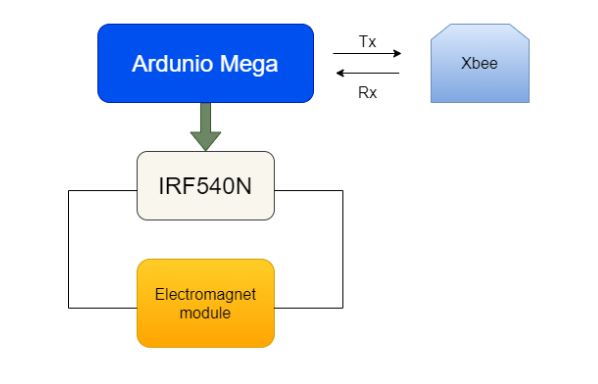
\includegraphics[width=0.6\textwidth]{irf540n.JPG}
    \caption{IRF540N Interfcing}
    \label{fig:robot}
\end{figure}


\EA
%%%%%%%%%%%%%%%%%%%%%%%%%%%%%%%%%%%%%%%%%%%%%%%%%%%%%%%%%%%%%%%%%%
\end{document}